\chapter{Semantic SLAM}

\section{DeLS-3D: Deep Localization and Segmentation with a 2D Semantic Map\cite{WangWang2018DeLS}}

\subsection{Abstract}

Sensor fusion scheme: Integrates camera videos, Motion sensors (GPS/IMU), and a 3D semantic map.

步骤:
\begin{itemize}
\item Initial Coarse camera pose obtained from consumer-grade GPS/IMU
\item A label map can be rendered from the 3D semantic map.
\item Rendered label map and the RGB image are jointly fed into a pose CNN, yielding a corrected camera pose.
\item A multi-layer RNN is further deployed improve the pose accuracy
\item Based on pose from RNN, a new label map is rendered
\item New label map and the RGB image is fed into a segment CNN which produces per-pixel sematnic label.
\end{itemize}

从结果可以看出,Scene Parsing以及姿态估计两者可以相互改善,从而提高系统的鲁棒性以及精确度。

\subsection{Introduction}

在Localization中,传统的做法是基于特征匹配来做,但这样的坏处是,如果纹理信息较少,那么系统就不稳定,会出错。一种改进办法是利用深度神经网络提取特征。实际道路中包含大量的相似场景以及重复结构,所以前者实用性较差。

在Scene Parsing中,深度神经网络用的很多,最好的基于(FCN + ResNet)的途径。在视频中,可以借助光流信息来提高计算速度以及时间连续性。对于静态场景,可以借助SfM技术来联合Parse以及Reconstruction.但这些方法十分耗时。

相机的姿态信息可以帮助3D语义地图与2D标签地图之间的像素对应。反过来,场景语义又会帮助姿态估计。

\subsection{Framework}

总的工作流程,如图\ref{DeLSFramework}所示:
\begin{figure}
\centering
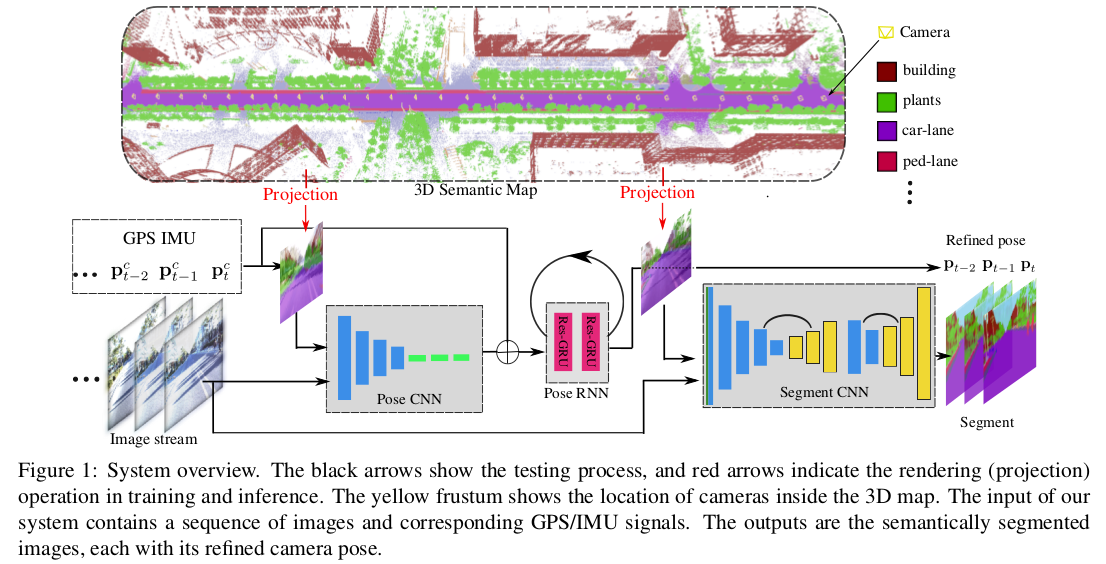
\includegraphics[width=0.95\textwidth]{SemanticSLAM/DeLS1.png}
\caption{DeLS Framwork}
\label{DeLSFramework}
\end{figure}

从图中可以看出,RGB Images 以及 根据GPS/IMU获得的semantic label map被输入到Pose CNN,然后输出的Pose信息输入到Pose RNN来对Pose进一步提高,{\bfseries 这里用RNN来获得前后帧的一致性}!然后在利用新得到的Pose来获取更精确的Semantic Label Map,最后,这个label Map以及RGB图像输入到Segment CNN来进一步提高语义地图的精度。这里标签地图被用于提高语义地图的空间精度以及时间一致性。

网络的训练是基于非常精确地相机姿态以及语义分割,所以可以采用监督学习。

\subsection{Related Work}

\begin{itemize}
\item Camera Pose Estimation

\begin{itemize}
\item PnP

在大的范围内,可能需要提供姿态的先验信息。但对于城市环境中存在大量的Points,这种方法不适用,且不适用于纹理少、结构重复、以及重叠的区域。

\item Deep learned features

PoseNet, LSTM-PoseNet, Bi-Directional LSTM, or Kalman filter LSTM.但实际中由于存在植被等重复性的场景,所以十分有必要加入GPS/IMU等信息来获得鲁棒的定位结果。而在这里,我们采用结合RGB图像与Online Rendered label map的方式来提供更好的结果。

{\bfseries \color{red} 这里问题来了,首先是label map的精度如何?其次,随着时间的变化,label map与实际RGB图像可能完全不同,如季节改变了,这应该如何?}

\end{itemize}

\item Scene Parsing

FCN, Multi-scale context module with dilated convolution, Pooling, CRF, or Spatial RNN with hundreds of layers.这些方法都太耗时了。

一些方法是利用小模型或者模型压缩来加速,但会降低精度。

当输入是Video时,需要考虑时空信息。当前,存在利用光流来帮助label以及semantic在相邻帧之间的传递。借助3D信息以及相机姿态把相邻帧联系起来,可以更好的处理静态背景下的表示。具体的,是使用DeMoN来提高推理效率。

\item Joint 2D-3D for video parsing

CNN-SLAM把传统的3D重建模块替换为深度预测网络,且借助语义分割网络来获取场景语义。同样比较耗时、仅适合静态背景,重建效果也不好。

\end{itemize}

\subsection{Dataset}

\begin{itemize}
\item Data collection

Mobile LIDAR to collect point clouds of the static 3D map. Cameras' resolution: 2018 * 2432.

\item 2D and 3D Labeling

\begin{itemize}
\item Over-segment the point clouds into point clusters based on spatial distances and normal directions, then label each point cluster manually.

\item Prune out the points of static background, label the remaining points of the objects.

\item After 3D-2D projection, only moving object remain unlabeled.

\end{itemize}

\item 使用图形学中的 \textit{Splatting techniques} 来优化未被标签的像素。

\end{itemize}

\subsection{Localizing camera and Scene Parsing}

\subsubsection{Render a label map from a camera pose}

初始的相机的姿态来自于GPS/IMU等传感器。

6-DOF相机姿态:$\mathbf{b} = [\mathbf{q}, \mathbf{t}] \in SE(3)$. 其中$\mathbf{q} \in SO(3)$是四元数表示的旋转,$\mathbf{t} \in \mathbb{R}^3$表示Translation。

在由Point经Spaltting获取其面时,面积大小$s_c$根据Point所属的类别来决定,且与该类别与相机的平均距离的比例有关。

\begin{displaymath}
s_c \propto \frac{1}{|\mathcal{P}_c|}\sum_{x \in \mathcal{P}_c}\min_{\mathbf{t}\in \tau}d(x, t)
\end{displaymath}

其中,$P_c$是属于类别$c$的3D点云,$\tau$是精确地相机姿态。如果面积过大,则会出现Dilated edges,而如果面积过小,则会形成Holes。

\subsubsection{Camera Localization rectification with road prior}

\textbf{CNN-GRU pose Network Architecture}

文中的Pose Network包含一个Pose CNN以及一个Pose GRU-RNN。其中Pose CNN的输入是RGB图像I以及一个标签地图L。输出是一个7维的向量,表示输入图像I与输入标签地图L(由较粗糙的姿态$\mathbf{p}_i^c$得到)之间的位姿关系,从而得到一个在3D Map中更精确的姿态:
$\mathbf{P}_i = \mathbf{p}_i^c + \hat{\mathbf{p}}_i$。

CNN结构借鉴DeMoN,利用打的Kernel Size来获取更大的内容,同时保证运行效率,减少参数量。

由于输入的是图像流,为了保证时间一致性,所以在Pose CNN之后又加上一个多层的GRU网络,且该网络具有Residual Connection的连接结构。结果表明,RNN相比于卡尔曼滤波可以获得更好的运动估计。

\textbf{Pose Loss}

类似于PoseNet的选择,使用Geometric Matching Loss来训练。

\subsubsection{Video Parsing with Pose Guidance}

上一步得到的Pose估计,不是完美的,因为存在light poles存在。由于反光,很多点消失了。此外,由于存在动态物体,这些物体可能在原来的标签地图中不存在,所以这些区域可能发生错误。因此,利用额外的一个Segment CNN来出来这些问题。且利用标签地图来指导分割过程。

\textbf{Segment Network Architecture}

首先基于RGB图像对该网络训练,然后加入标签地图数据进行微调(Fine Tune).具体结构如图\ref{SegmentDeLS}所示。

\begin{figure}[!hbtp]
\centering
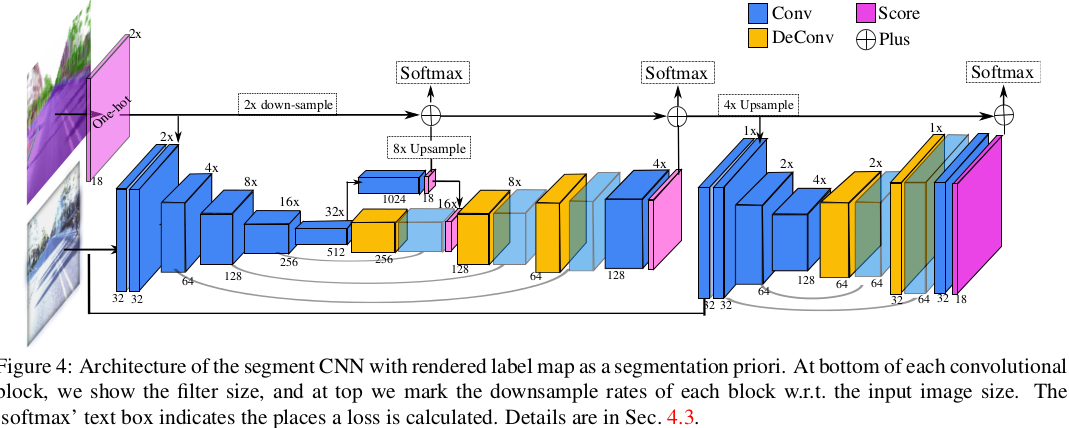
\includegraphics[width=0.95\textwidth]{SemanticSLAM/DeLS2.png}
\caption{Segment Network in DeLS}
\label{SegmentDeLS}
\end{figure}

需要注意的是,当标签地图加入框架时,需要经过编码,即每一个像素经One-hot操作得到一个32维的Feature Representation。然后得到的32维特征加入到RGB图像的第一层卷积输出中,且该层的Kernel数也是32个,从而平衡了两种数据的通道数(Channel Number)。

\subsection{Experiment}

\begin{itemize}
\item Adopt OpenGL to efficiently render a label map with the z-buffer handling. 

\item Implement all the networks by adopting the MXNet platform.

\item 使用RNN可以提高Pose的精度,也可以提高Segment的精度,尤其对于纤细的物体。

\end{itemize}

\subsection{Conclusion}

基于已有的3D语义地图以及视频数据,实现相机的姿态、场景语义任务的实现。算法融合了多种传感器信息。实验表明,相机位姿估计与场景语义两类任务可以相互促进、提高。

\section{PAD-Net: Multi-Task Guided Prediction-and-Distillation Network for Simultaneous Depth and Scene Parsing \cite{Xu2018PADNet}}

\subsection{Abstract}

利用同一个网络,完成深度估计与场景解析两个任务。具体来说,通过神经网络学习一系列的中间辅助任务(Intermediate Auxiliary Tasks),然后基于中间任务的输出,作为多模式数据(Multi-modal  input)输入到下一层网络中,完成最终的深度估计以及场景解析两个任务。

其中,一系列的中间任务包括低层任务和高层任务。低层任务包括:Surface Normal, Contour;高层任务包括:Depth Estimation, Scene Parsing.

\subsection{Analysis}

\subsubsection{Effect of Direct Multi-task Learning}
It can be observed that on NYUD-v2, the Front-end + DE + SP slightly outperforms the Front-end
+ DE, while on Cityscapes, the performance of Front-end + DE + SP is even decreased, which means that using a direct multi-task learning as traditional is probably not an effective means to facilitate each other the performance of different tasks. (DE: Depth Estimation, SP: Scene Parsing)

\subsubsection{Effect of Multi-modal Distillation}
这种Multi-Modal Distillation对结果十分有效。且:
\begin{quote}
By using the attention PAD-Net (Distillation C + SP) guided scheme, the performance of the module C is further improved over the module B.
\end{quote}

\subsubsection{Importance of Intermediate Supervision and Tasks}

测试了选择不同的中间任务类型,如:(Multi-Task Deep Network)MTDN + inp2(depth + semantic map), MTDN+3inp3(depth + semantic + surface normal), MTDN + all(depth + semantic + surface + contour).

其中MTDN + all比MTDN + 0-3都好。

\section{RNN for Learning Dense Depth and Ego-Motion from Video}

参考文献:\cite{Wang2018DenseSLAMNet}

{\color{red}时间:2018年05月19日}

\subsection{Abstract}

现在基于学习的单目深度估计,在Unseen Dataset上泛化较差,可以利用连续两帧之间的特征匹配来解决。本文提出了基于RNN的多目视觉深度估计以及运动估计。结果表明,在远距离上的深度估计,表现很好。本文方法可使用both static and deformable scenes with either constant or inconsistent light conditions.

\subsection{Introduction \& Related Works}

由于CNN只能捕获单帧内部的空间特征,所以即使输入两帧图像,实际效果也比较差。相关的SLAM框架有:

\begin{itemize}
\item ORB-SLAM, DSO: 稀疏SLAM
\item LSD-SLAM: semi-dense SLAM,利用光强来实现跟踪以及构建地图
\item DTAM: dense SLAM
\end{itemize}

上述框架仅适用于静态、光照恒定、足够的camera motion baseline的情景。

进来,CNN可被用于SLAM中的以下部分:
\begin{itemize}
\item Correspondence matching
\item Camera Pose estimation
\item Stereo
\end{itemize}
输出包括:
\begin{itemize}
\item Depth maps
\item point clouds and voxels
\end{itemize}
CNN的优势在于可以适用于纹理较少、表面覆盖、很细等场景下,这些场景对纯使用几何技术来说很难实现。

Newcombe研究表明,多目视觉有助于提高深度估计的精度,而本文作者认为采用相邻几帧可以实现类似的效果。

有作者利用一个非监督生成模型来学习复杂的3D到2D的投影。但这些手段不太适用于Deformable Objects.

\subsection{Network Architecture}

\begin{figure}[!htbp]
\centering
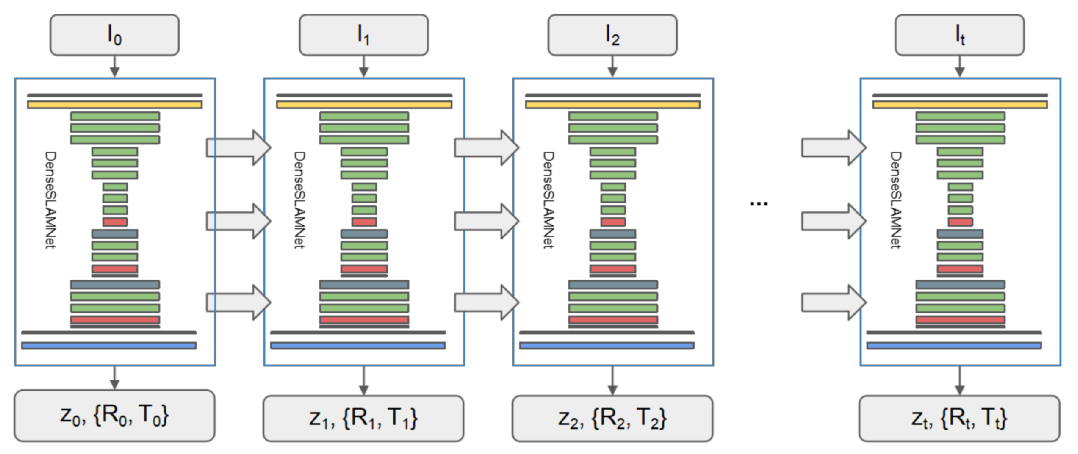
\includegraphics[width=0.95\textwidth]{SemanticSLAM/DenseSLAMNet1.png}
\caption{Dense SLAM框架}
\label{DenseSLAMNet1}
\end{figure}

从图\ref{DenseSLAMNet1}可以看出,它接受当前RGB图像$I_t$以及来自迁移级的隐藏状态$h_{t-1}$。$h_{t-1}$通过LSTM单元进行内部转移。网络的输出是稠密地图$z_t$以及相机的姿态$R_t, T_t$等。有没在每一时刻,只输入一帧图像,且输出该帧对应的深度以及姿态,所以相比于CNN具有更高的灵活性。

具体的每一块的细节结构如下:

\begin{figure}[!htbp]
\centering
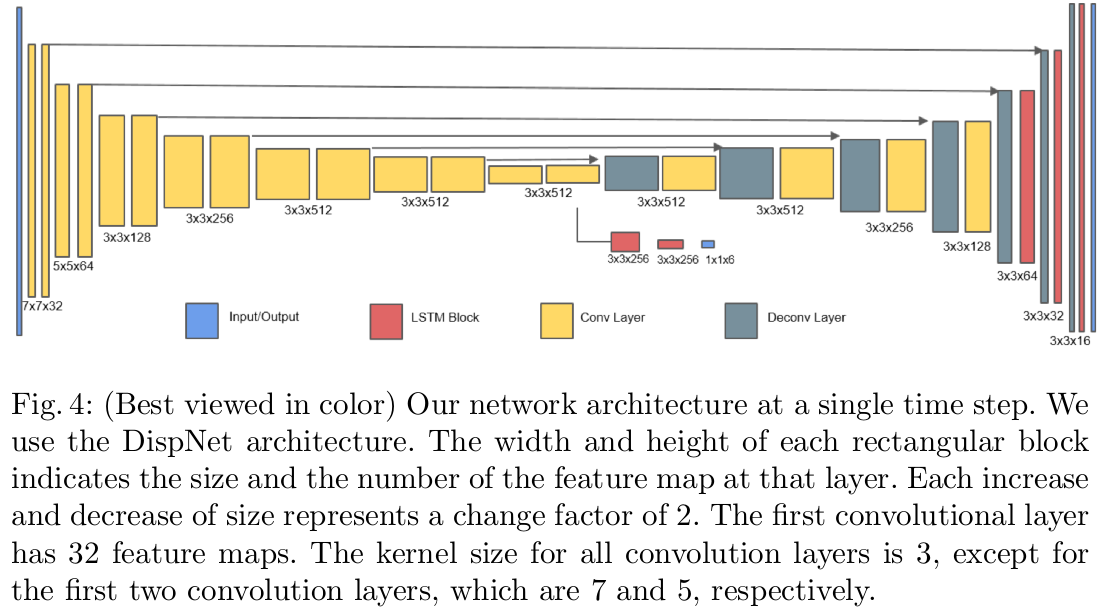
\includegraphics[width=0.95\textwidth]{SemanticSLAM/DenseSLAMNet2.png}
\caption{Dense SLAM中每一级的细节框架}
\label{DenseSLAMNet2}
\end{figure}

网络结构的另一个参数是时间窗口的大小$N$。本文中$N=10$,也就是说,图\ref{DenseSLAMNet2}中的结构被重复十次。

\subsection{Training}

During training, we feed
frames to the network and compute losses from all frames in a temporal window. However, there is no input length constraint at test time.

\subsubsection{Loss Function}

由三部分组成:
\begin{itemize}
\item A Point-wise depth loss

\begin{displaymath}
L_{depth} = \sum_{t}^{N}\sum_{i, j}\left\| \xi_t(i, j) - \hat{\xi}_t(i, j) \right\|_{L1}
\end{displaymath}
其中,$i, j$为索引,$t$为time step.使用$L1-Norm$的原因是,它对噪声更鲁棒。

\item a camera pose loss

Use the Euler angle $R$ 和平移向量$T$。

\begin{displaymath}
\begin{gathered}
L_{rot} = \sum_{t}\left\| r_t - \hat{r}_t \right\|_2 \\
L_{trans} = \sum_{t}\left\| t_t - \hat{t}_t \right\|_2
\end{gathered}
\end{displaymath}

\item a scale-invariant gradient loss

为了保证深度图的Smoothness和Sharpness,所以增加了这个loss。具体如下:
\begin{displaymath}
L_{grad} = \sum_{t}\sum_{h\in\{ 1, 2, 4, 8, 16 \}}\sum_{i, j}\left\| g_{h, t}(i, j) - \hat{g}_{i, j}(i, j)\right\|_2
\end{displaymath}
其中,$h$代表不同的尺度。$g_{h, t}$is a scale-normalized, discretized measurement of the local changes of $\xi_t$。定义如下:
\begin{displaymath}
g_{h, t} = \left( \frac{\xi_t(i+h, j) - \xi_t(i, j)}{|\xi_t(i + h, j) + \xi_t(i, j)|}, \frac{\xi_t(i, j+h) - \xi_t(i, j)}{|\xi_t(i, j+h) + \xi_t(i, j)|}    \right)
\end{displaymath}

$L_{grad}$emphasizes the depth discontinuities, such as occlusion
boundaries and sharp edges, as well as the smoothness in homogeneous regions.
This property encourages the estimated depth map to preserve more details and
reduce noise. Therefore, we put highly weight on this component of the loss. 这一项在所有的Loss中比重较大。

\end{itemize}

最终的Loss由上面几项的和构成:
\begin{displaymath}
L = \alpha * L_{depth} + \beta * L_{pose} + \gamma * L{grad}
\end{displaymath}
其中,$\alpha, \beta, \gamma$是系数,由经验决定。


注意,下面解释的是为什么使用Disparity而不是直接使用深度。
\begin{quote}
{\color{red} \textbf{Caution!} Disparity, the reciprocal of depth (深度的倒数), $\xi = \frac{1}{z}$  as our direct estimation because it can represent points at infinity and account for the localization uncertainty of points at increasing
distance.}
\end{quote}

Different datasets have different camera intrinsic parameters, so we
explicitly crop and resize images to ensure uniform intrinsic parameters. This
step assures that the non-linear mapping between color and depth is consistent
across all training datasets.

\subsection{Experiments}

We evaluate DenseSLAMNet using five error metrics。具体可以参考文章。
\begin{itemize}
\item Sc-inv
\item Abs-rel, Abs-inv
\item RMSE, RMSE-log
\end{itemize}

\subsection{Ablation Studies}

比较了三种不同的网络结构。
\begin{enumerate}
\item CNN-SINGLE, 去掉图\ref{DenseSLAMNet2}中LSTM单元
\item CNN-STACK, 使用与CNN-SINGLE相同的网络,但是输入stack of ten images as input.
\end{enumerate}

实验结果表明,LSTM可有效保留时间域的信息,从而深度预测的更好。

\subsubsection{Conclusions}

引入了LSTM单元。
Our method effectively utilizes the temporal relationships between neighboring
frames through LSTM units, which we show is more effective than simply stack-
ing multiple frames together as input.

比几乎所有的单帧CNN-based 都好。
Our DenseSLAMNet outperformed nearly
all of the state-of-the-art CNN-based, single-frame depth estimation methods on
both indoor and outdoor scenes and showed better generalization ability.


\section[DA-RNN]{DA-RNN: Semantic Mapping with Data Associated Recurrent Neural Networks}

参考文献:\cite{Xiang2017DARNN}

{\color{red} \textbf{评语} 看得出来,RNN在帮助建立相邻帧之间的一致性方面具有很大的优势。}

本文利用可以实现Data Associate的RNN产生Semantic Label。然后作用于KinectFusion,来插入语义信息。

所以本文利用了RNN与KinectFusion来实现语义地图的构建!

\subsection{Related Works}

{\bfseries 本文提出的 DA-RU (Data Associated Recurrent Unit) 可以作为一个单独的模块加入到已有的CNN结构中!}

\subsection{Methods}

需要注意到是,本文采用了DA-RNN与KinectFusion合作的方式来产生最终的Semantic Mapping,而文章采用的则是ORB-SLAM与CNN结合,他们有一些共同的结构,如Data Associate,虽然我现在还不明白这个DA具体得怎么实现!?

\subsection{Experiments}

实验表明,针对不同的实验输入场景,RGB图像和Depth图像可能发挥不同的作用,有一些时候甚至让结果更差,而本文采用Contatenated把来自于RGB和Depth的Feature进行组合起来,在这里,是否可以采取Attention或者\cite{Xu2018PADNet}中采用的Knowledge Distillation的方式进行多模态数据融合呢!?

此外,实验中也发现,有时候RGB图像的Color会影响实验结果,所以,是否可以利用一些其它的不那么Confusing的数据呢,比如Shape等,这也类似于\cite{Xu2018PADNet}中多任务中的Contour类似吧!


\subsection{Conclusion}

\begin{itemize}
\item $\star$将来的可以借助Optical Flow来生成图像帧之间的Data Associate,来代替KinectFusion的作用!
\end{itemize}

\section{SemanticFusion: Dense 3D Semantic Mapping with CNNs}
参考文献:\cite{SemanticFusion2016}

主要框架,用到了ElasticFusion和CNN来产生稠密的Semantic Mapping.

\subsection{Introduction \& Related Works}

本文的算法,利用SLAM来实现2D Frame与3D Map之间的匹配(Corresponding)。通过这种方式,可以实现把CNN的语义预测以概率的方式融合到Dense semantically annotated map.

为什么选择ElasticFusion呢,是因为这种算法是surfel-based surface representation,可以支持每一帧的语义融合。

比较重要的一点是,通过实验说明,引入SLAM甚至可以提高单帧图像的语义分割效果。尤其在存在wide viewpoint variation,可以帮助解决单目2D Semantic中的一些Ambiguations.

之前存在方法使用Dense CRF来获得语义地图。

本文的主要不同是:利用CNN来产生语义分割,然后是在线以 Incremental 的方式生成Semantic Map。即新来一帧就生成一帧的语义地图。

\subsection{Method}

系统由三部分组成:
\begin{itemize}
\item A real-tiem SLAM system ElasticFusion

用于提供帧间的关联、全局一致的地图

\item CNN

产生语义分割

\item Bayesian update scheme

基于SLAM提供的Pose关系、CNN提供的每个像素的Class Probability对Map中的每一个surfel的Class Probability进行更新!

\end{itemize}

此外,作者还尝试了用CRF来利用SLAM提供的Geometry帮助语义分割。

非常粗糙的流程图如下图所示:
\begin{figure}[!hbtp]
\centering
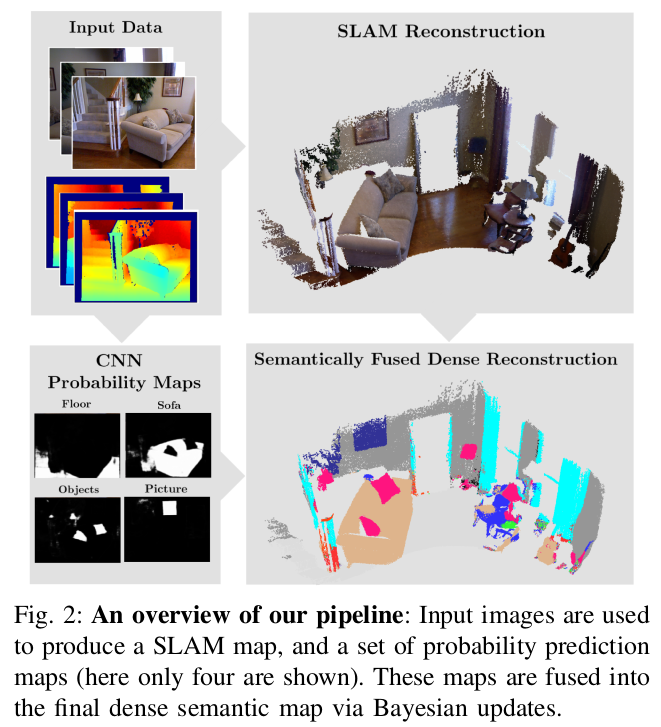
\includegraphics[width=0.75\textwidth]{SemanticSLAM/SemanticFusion0.png}
\caption{粗糙的数据流图}
\label{SemanticFusion0}
\end{figure}

\subsubsection{SLAM Mapping}
就是使用ElasticFusion.

\subsubsection{CNN Architecture}

使用Deconvolutional Semantic Segmentation network,与FCN同年提出的另一个分割网络。

在本实验中,输入由RGB变为RGBD,多了一个Channel.然而,深度相关的训练数据比较少,为了提高利用率,作者利用其它三个输入的光强的平均值对Depth Filter进行初始化。

对输入数据,作者还进行了Scaling, RGB是用Bilinear Interpolation, Depth数据是Nearest enighbour。

\subsubsection{Incremental Semantic Label Fusion}

在生成的地图$\mathcal{M}$中,每一个Surfel(ElasticFusion的结果)不仅代表了Location、Normal等信息,还包含一个类别($\mathcal{L}$)的分布。

输入数据为$\mathbf{I}_k$表示RGB图像与Depth等。

在对每一个Surfel进行类别分布概率更新时,采用的Recursive Bayesian update,这个算法就是Probability Robotics里面最基础的算法,也就是分为Prediction和Correlation两个步骤。

\begin{displaymath}
P(l_i | I_{1, \ldots, k}) = \frac{1}{Z}P(l_i | I_{1, \ldots, k- 1})P(O_{u(s, k)=l_i | I_k})
\end{displaymath}

其中,第一个$P$表示根据过去的信息的预测,在这里也就是已有的$\mathcal{M}$里面的一个surfel的class probability,如果,是一个全新的Surfel,则初始化它为均匀分布,因此这样熵最大;而第二个$P$表示来自CNN输入是$I_k$时输出的class probability,然后对已有地图中的surfel的class probability进行Correlation!

\subsubsection{Map Regularisation}

作者尝试了利用CRF来借助map geometry对预测的Semantic surfel进行Regularise。

在这里,把每一个Surfel当做CRF的一个Node。

这一部分,参考论文吧。

\subsection{Experiments}

本文用到的Semantic分割的方法(CNN + SLAM)与普通的单CNN相比,具有很大的优势。本文的方法是,得到3D的Semantic Map后,重投影到2D图像中。

时间方面,SLAM需要29.3ms,CNN的前向传播用了51.2ms,Bayesian更新用了41.1ms。

\subsection{总结}

未来也还是SLAM与语义分割相互促进吧,达到Semantic SLAM。


\section{Meaningful Maps with Object-Oriented Semantic Mapping}
参考文献:\cite{Meaningful2016}

主要的框架是,利用CNN与ORB-SLAM2来实现Semantic Mapping。{\bfseries 但是都用到了Data Association的操作}!而且本文还是Object-oriented (Instance level) !

\subsection{Introduction \& Related Works}

{\bfseries 重要:}

与已有的方式不同的是,本文的算法不仅分割独立的3D Point,也就是把语义信息投影到3D Point中,而是投影到3D Structure。这样会更有利于场景理解。

已有的SLAM算法得到的结果都是一些几何上的概念,比如:点、面、表面等。另一方面,为了实现与环境交互,必须基于语义地图才行。

\subsubsection{Semantic Mapping}

语义信息与地图构建可能属于两个不同的过程得到。

有一些算法用到了HMM或Dense CRF等。

\subsubsection{Object Detection and Semantic Segmentation}

FCN的缺点是,形成的语义地图一般缺少Notion of independent object instances. 如果只是Pixel-level的labels不能辨别有重叠时物体的身份。

也有一些Instance-level的分割算法,但精度、速度都有待提高。

\subsection{Object Oriented Semantic Mapping}

算法的主要步骤:
\begin{figure}[!hbtp]
\centering
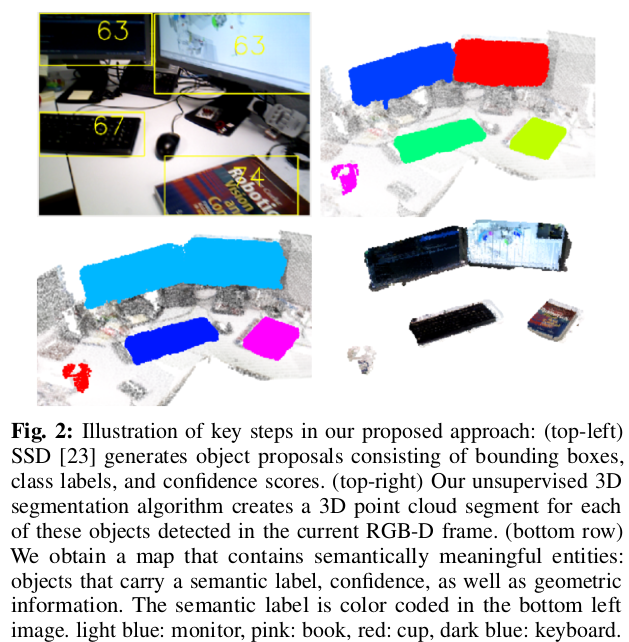
\includegraphics[width=0.75\textwidth]{SemanticSLAM/OrientedMap0.png}
\caption{算法的几个主要步骤}
\label{OrientedMap0}
\end{figure}

算法使用RGB-D作为输入,算法是用ORB-SLAM2提供相机的姿态、地图等。

\subsubsection{Object Detection for Semantic Mapping}

本文使用SSD来完成Object的Location和 Recognition。

\subsubsection{3D Segmentation}

由于需要非常精确的图像分割,所以本文利用Depth图来帮助分割。所以需要对Depth进行分割的算法,本文采用了文章\cite{Felzenszwalb2004}\cite{Pham2016Geometrically}等人的算法。也是涉及到基于图的分割的过程。

\subsubsection{Data Association}

重点。

当完成了把3D Point投影到识别的物体后,数据关联要做的事:判断检测到的物体是否已经在已经构建的地图中存在了呢,如果不存在的话,就需要新增这个物体。

通过一个二阶的流程来实现:

\begin{itemize}
\item 对于每一个检测到的Object,根据点云的欧式距离,来选择一系列的Landmarks(已经检测到并在地图里面已经有的Object)
\item 对Object和Point Cloud of landmark进行最近邻搜索,使用了k-d tree来提高效率,其实这一步也就是判断当前图像检测到的Object与已有的地图中的Landmark(Object)是否相匹配。
\end{itemize}

在第二步中,如果多余50 \% 的Points的都距离小于2cm的话,就说明这个检测到的Object已经存在了。

这个也就是把CNN的分割结果与地图中的Object进行关联起来,并用颜色表示Map中Object的类别。

\subsubsection{Object Model Update}

地图中的目标保存:
\begin{itemize}
\item 与目标相关联的分割的3D点云
\item ORB-SLAM中因子图的各个位姿的索引
\item 有SSD提供的各个目标的置信度
\end{itemize}

\begin{figure}[!hbtp]
\centering
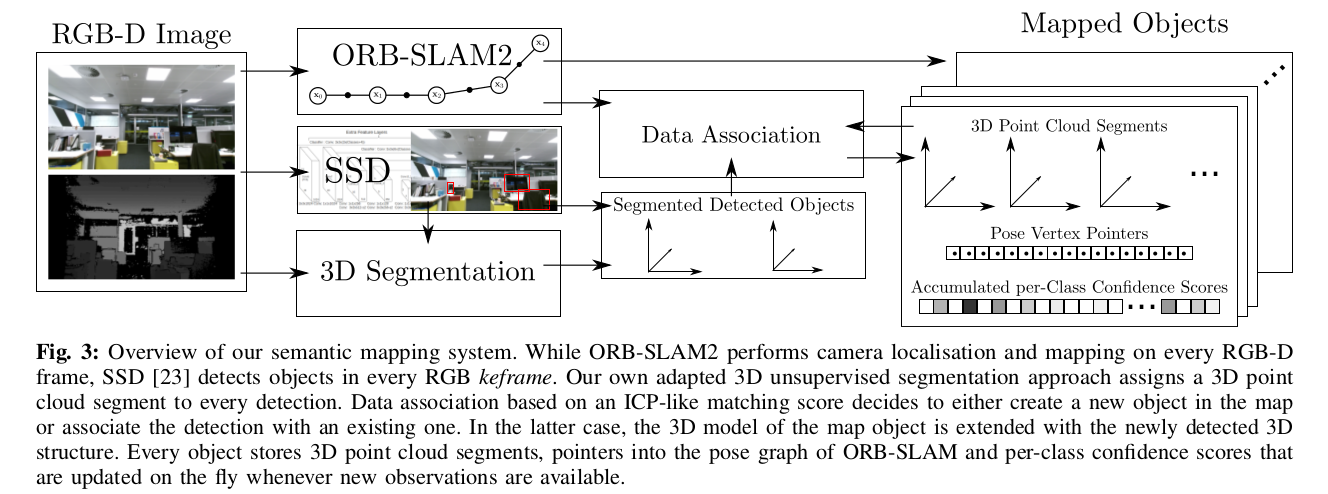
\includegraphics[width=0.95\textwidth]{SemanticSLAM/OrientedMap1.png}
\caption{Semantic Mapping 系统概览}
\label{OrientedMap1}
\end{figure}

上图中可以看出,


{\color{red} \textbf{评语}:在上一篇SematicFusion中,采用的Recursive Bayesian 的更新规则来完成地图更新的!看来,这个是CNN与传统的SLAM框架结合的时候的一个需要解决的问题,那就是如何把新来的物体与已有的地图中的物体相互关联起来,并更新!}

\subsubsection{Map Generation}

通过保存Keyframe中物体的3D poin clouds、每一个物体的3D分割以及执行位姿图中的一个指针。

\subsection{总结}

未来可以的发展方向:
\begin{itemize}
\item 语义Landmark如何提高SLAM的精度,从而实现Semantic SLAM
\item 把稀疏的语义地图改进为稠密地图
\end{itemize}

\section[LiteFlowNet]{LiteFlowNet: A Lightweight Convolutional Neural Nework for Optical Flow Estimation}

参考文献:\cite{Hui2018LiteFlowNet}, CVPR 2018

\subsection{背景知识}

FlowNet2是基于CNN进行光流估计的SOTA算法(?), 需要160M的参数量。LiteFlowNet实现了30倍的轻量化,并且比FlowNet2块1.36倍。

主要的贡献:
\begin{itemize}
\item 在每一层金字塔(Pyramid Level)预测光溜更高效的轻量级联网络。通过早前矫正(Early Correction)提高了精度,同时无缝支持网络中的描述子匹配。
\item 提出了一个新型的光流正则化层,可以改善野值点、光流边界模糊等问题,是基于特征驱动的区域卷积实现
\item 网络结构可以高效提取Pyramidal Feature以及Feature Warping,而不是像FlowNet2中的Image Warping。
\end{itemize}

FlowNet2通过级联FlowNet,来不断调优光流场, by contributing on the flow increment between the first image and the warped second imaeg?

后来,SPyNet通过在每一Pyramid level采用Imae Warping实现了只有1.2M大小的网络,但精度只有FlowNet大小,而达不到FlowNet2的水平。

{\bfseries Image Warping: 图像扭转,是一种数字图像处理过程,在任何图像中所描述的任何形状都会产生显著有损。扭曲可用于矫正图像有损,同时可用于某种创意目的。纯粹的图像扭曲意味着点到点的映射,而不改变其颜色。}

提高FlowNet2以及SPyNet的两种准则(Principles):

\begin{itemize}
\item Pyramid feature extraction

Consists of an encoder and a decoder. Encoder把输入的图像对分别映射到多尺度高维特征空间中;Decoder以Coarse-to-fine的框架估计光流场。这比FlowNet2采用U-Net更轻量化。相比于SPyNet,我们的模型把特征提取与光流估计两个过程分离,可以更好的处理精度与复杂度之间的矛盾。

\item Feature Warping

FlowNet2与SPyNet将输入图像对中的第二幅图像基于先前估计的光流进行Warp,然后使用Warped的第二幅图像与第一幅图像的特征图谱Refine估计的光流。

所以这个过程中,首先把第二幅图像进行Warp,然后提取Warp图像的特征,这个过程十分繁琐。所以,本文提出直接对Feature Map进行warp。保证模型更精确以及高效。

\end{itemize}

更详细的细节一定要看原文\cite{Hui2018LiteFlowNet}。

此外,除了上面两个主要改进的 Principle, 作者还提出第三个比较重要的改进措施,那就是 Flow Regularization.

\begin{itemize}
\item Flow Regularization

级联的光流估计类似于能量最小化方法中的保真度(Data Fidelity)的作用。 为了消除边界的模糊以及野值点,Regularize flow Field的常用Cues:
\begin{itemize}
\item Local flow consistency
\item Co-occurrence between flow boundaries
\item Co-occurrence between intensity edges
\end{itemize}

对应的代表方法包括:
\begin{itemize}
\item Anisotropic image-driven
\item image- and flow-driven
\item Complementary regularizations
\end{itemize}

在本文中,提出的是Feature-driven local convolution layer at each pyramid level. 该方法对Flow-以及Image-敏感。

{\color{red} \textbf{评语}:看起来,一个是提高精度,一个是提高效率,这是两个最终的目的。提高精度可以通过设计网络结构以及增加其它考虑来实现;提高效率的一个重要表现是降低模型的参数数量,提高运算速度。不过,本文虽然参数数量减少了30倍,但速度却只提高了1.36倍,这里面的原因是什么?}

\end{itemize}

\subsection{Related Works}

\subsubsection{Variational Methods}

Address illumination changes by combining the brightness and gradient constancy assumptions.

DeepFlow, propose to correlate multi-scale patches and incorporate this as the matching term in functional.

PatchMatch Filter, EpicFlow.

本文提出的网络结构,是受Variational methods中的Data Fidelity以及正则化启发。

\subsubsection{Machine Learning Methods}

PCA-Flow. 这些参数化模型可以通过CNN高效的实现。

\subsubsection{CNN-based Methods}

FlowNet, 使用能量最小化作为后处理步骤,来降低在光流边界的平滑效应。不能端到端训练?

FlowNet2, 通过FlowNet的级联实现。虽然提高了精度,但模型更大,计算更复杂。

SPyNet,受Spatial Pyramid启发,模型更紧凑,但效果远不如FlowNet2。

InterpoNet, 借助第三方系数光流但需要off-the-shelf的边缘检测。

DeepFlow, 使用Correlation而不是真正意义的CNN,参数不能训练。

\subsubsection{Establish Point Correspondence}

Establishing point correspondence, 一种方式是Match Image Patches

CNN-Feature Matching, 首先被Zagoruyko等人提出(Learning to compare image patches via CNN, 2015 CVPR)。

MRF-based, G$\ddot{u}$ney等人提出利用Feature Representation以及利用MRF来估计光流。

Bailer使用多尺度Feature,然后以类似于Flow Fields的方式进行特征匹配。

Fischer和Ilg等人为了提高计算效率,仅在稀疏空间维度进行特征匹配。

本文中,We reduce the computational burden of feature matching by using a short-ranged matching of warped CNN features at sampled positions and a sub-pixel refinement at every pyramid level.

类似于Spatial Transformer, 本文利用 f-warp layer来区分不同个Channel.本文的决策网络是一个更普用的Warping Network,可以用来Warp高层次的CNN Features,而不仅仅是对Image进行Warpping.


\subsection{LiteFlowNet}

整体结构如下:
\begin{figure}[!hbtp]
\centering
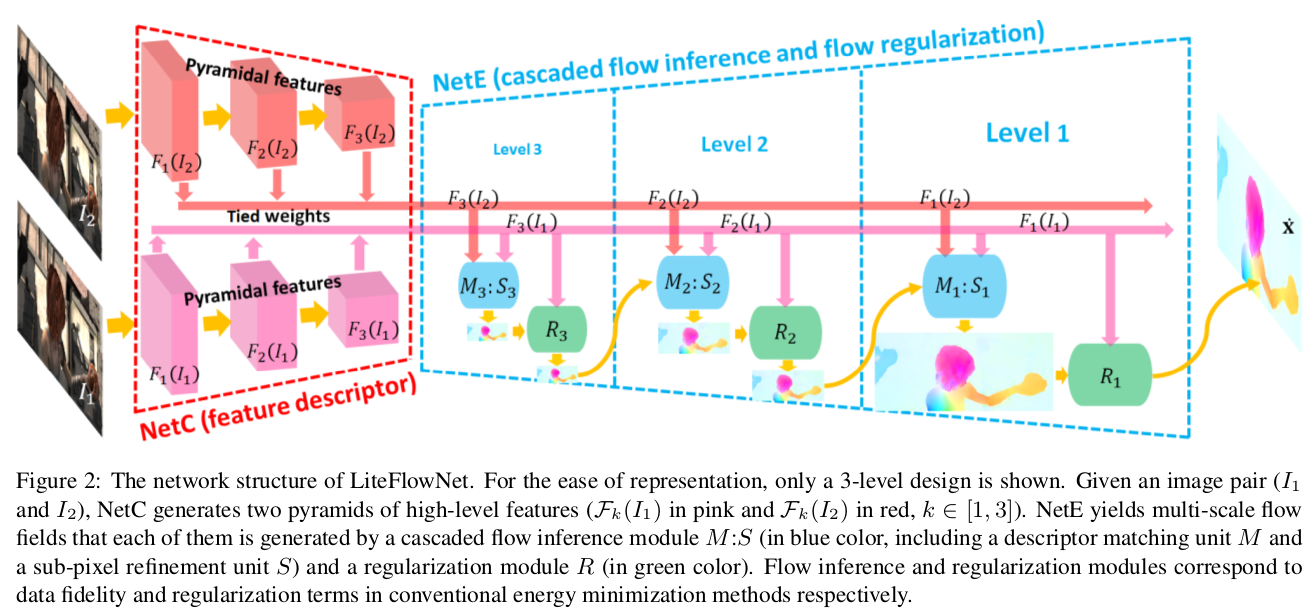
\includegraphics[width=0.95\textwidth]{SemanticSLAM/LiteFlowNet0.png}
\caption{LiteFlowNet结构框图}
\label{LiteFlowNet0}
\end{figure}

\subsubsection{Pyramid Feature Extraction}

进行stride-$s$的卷积操作,得到的Feature Map表示为:$\mathcal{F}_k(I_i)$,即第$i$个图像的第$k$层Feature Map。简化写成 $\mathcal{F}_i$。

\subsubsection{Feature Warping (f-warp)}

假设\.x为预测的光流,则Feature Warping是指:
\begin{displaymath}
\tilde{\mathcal{F}}_2(x) \triangleq \mathcal{F}_2(x + \dot{x}) \sim \mathcal{F}_1(x) 
\end{displaymath}

注意,Warping是作用于$\mathcal{F}$上的,而不是输入图像上的。

为了使上述过程可以支持end-to-end训练,这里采用Bilinear Interpolation进行插值的技术实现Warping。Bilinear Interpolation是支持后向传播训练的!修改后Warping实现公式如下:
\begin{displaymath}
\tilde{\mathcal{F}} = \sum_{x_s^i \in N(x_s)} \mathcal{F}(x_s^i)(1-|x_s - x_s^i|)(1 - |y_s - y_s^i|)
\end{displaymath}

其中,$x_s = x + \dot{x} = (x_s, y_s)^T$是输入的源Feature Map中的坐标。$x$denotes the target coordinates of the regular grid in the interpolated feature map $\mathcal{F}$,$N(x)$代表the four pixel neighbors of $x_s$.

自己的理解:首先$x$是插值后 的图像索引,而$x_s = x + \dot{x}$是插值前Feature Map中对应Object Feature的$x$索引处的索引。$x_s^i$是在$x_s$周围的四个紧邻像素。也就是个Bilinear Interpolated.

\subsubsection{Cascaded Flow Interface}

{\color{red} \textbf{评语}:这一块看的比较吃力。为什么会吃力?因为新的概念么?那么作者为什么提出这么麻烦的概念呢?实际效果又怎么样呢?}

通过计算高层特征向量的Correlation来实现输入图像的点对应。

\begin{displaymath}
c(x, d) = \mathcal{F}_1(x) \cdot \mathcal{F}_2(x + d) / N
\end{displaymath}
这个公式跟FlowNet中的计算方式区别不大。只不过这里的$N$是指Feature的长度。

\begin{figure}[!hbtp]
\centering
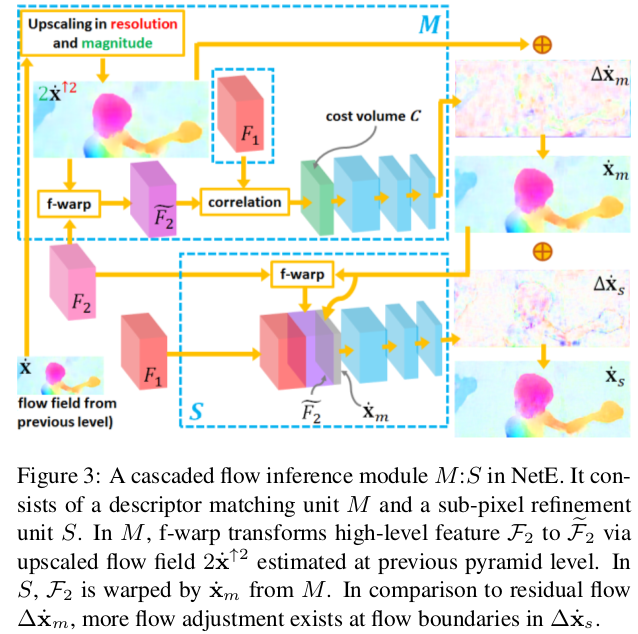
\includegraphics[width=0.75\textwidth]{SemanticSLAM/LiteFlowNet1.png}
\caption{在NetE中的级联光流推理模块,M:S}
\label{LiteFlowNet1}
\end{figure}

\textbf{M Module}$\;$  在Descirptor Matching unit M, Residual flow $\varDelta \dot{x}_m$. A complete flow field $\dot{x}_m$ is computed as follows, 这句话没懂

\begin{displaymath}
\dot{x}_m = \underbrace{M(C(\mathcal{F}_1, \tilde{\mathcal{F}}_2; d))}_{\varDelta \dot{x}_m} + s\dot{x}^{\uparrow s}
\end{displaymath}

其中,$\dot{x}$是上一层的最开始的光流估计!

\textbf{S Module}$\;$ 
为了进一步提高flow estimate  $\dot{x}_m$ 的精度,即达到亚像素级别。作者引入了Second flow inference。 这可以防止错误光流的放大并传到下一级。Sub-pixel refinement unit $S$,会产生一个更准确的光流场,这通过最小化$\mathcal{F}_1$和 $\tilde{\mathcal{F}}_2$之间的距离来实现。

\begin{displaymath}
\dot{x}_s = \underbrace{S(C(\mathcal{F}_1, \tilde{\mathcal{F}}_2, \dot{x}_m))}_{\varDelta \dot{x}_s} + \dot{x}_m
\end{displaymath}

{\bfseries 所以总的来说} M模块是为了计算$\varDelta \dot{x}_m$, 而$S$模块是为了计算$\varDelta \dot{x}_s$。对最开始$\dot{x}$估计的光流进行两次的Refinement.

\subsubsection{Flow Regularization}

这一部分主要消除光流边界的模糊、存在的artifacts等。提出用 feature-driven local convolution (f-lcon)

假设Feature Map (F)的尺寸为:$M * N * c$,定义f-lcon的滤波器为$\textbf{G}={g}$

对于输入为$\dot{x}_s$, Flow Regularization值的是:
\begin{displaymath}
\dot{x}_r = R(\dot{x}_s; G)
\end{displaymath}
输出的是正则化后的光流估计$\dot{x}_r$

下面的关键是如何生成这个用于正则化的卷积核。为此,作者定义了一个feature-driven的距离度量$\mathcal{D}$,总的来说,该度量由一个CNN unit $R_D$来计算:
\begin{displaymath}
\mathcal{D} = R_D(\mathcal{F}_1, \dot{x}_s, O)
\end{displaymath}

基于这个度量,可以计算得到卷积核:
\begin{displaymath}
g(x, y, c) = \frac{\exp(-\mathcal{D}(x, y, c)^2)}{\sum_{(x_i, y_i)\in N(x, y)}\exp(-\mathcal{D}(x_i, y_i, c)^2)}
\end{displaymath}

其中$N(x)$表示一个$\omega * \omega$的近邻。

\subsection{Ablation Study}

算法的结果是优于 FlowNet2, SPyNet等。

\subsubsection{Feature Warping}

没有Warping, 光流更Vague.通过计算residual flow (M:S两个模块的功能)可以提高估计效果。

M: Matching

S: Sub-pixel refinement

R: Regularization units in NetE

\subsubsection{Descriptor Matching}

\subsubsection{Sub-Pixel Refinement}

The flow field generated from
WMS is more crisp and contains more fine details than
that generated from WM with sub-pixel refinement dis-
abled.

更小的flow artifacts.

\subsection{Regularization}

In comparison WMS with regularization
disabled to ALL, undesired artifacts exist in homogeneous
regions

Flow bleeding and
vague flow boundaries are observed.

表明, Feature-driven local convolution对于光滑光流场、保持crisp flow boundaries非常重要!

\subsection{Conclusion}

Pyramidal feature extrac-
tion and feature warping (f-warp) help us to break the de
facto rule of accurate flow network requiring large model
size. To address large-displacement and detail-preserving
flows, LiteFlowNet exploits short-range matching to gener-
ate pixel-level flow field and further improves the estimate
to sub-pixel accuracy in the cascaded flow inference. To
result crisp flow boundaries, LiteFlowNet regularizes flow
field through feature-driven local convolution (f-lcon). With
its lightweight, accurate, and fast flow computation, we ex-
pect that LiteFlowNet can be deployed to many applications
such as motion segmentation, action recognition, SLAM,
3D reconstruction and more.


\section{小结}

2018.05.23小结

在生成Semantic Map的时候,看样子现在的趋势,是利用RNN保证时间一致性;利用多模态数据提高精度,但如何融合多模态数据的Feature有待研究,现有的有一些是直接Concatenate、Knowledge Distillation、Attnetion(?)等机制。


\section{ExFuse: Enhancing Feature Fusion for Semantic Segmentation}

参考文献:\href{https://zhuanlan.zhihu.com/p/37177073}{ExFuse简介-知乎}

\subsection{要解决的问题}

在语义分割领域中,经常需要融合多层的Feature。然而,底层的Feature含有的语义信息较少,但分辨率较高,噪声也比较少,这是由于卷积层比较浅;而高层的Feature语义信息多,但空间分辨率很小。

所以本文就提出了:1)增加底层特征的语义;2) 在高层中增加空间信息

\subsection{Method}

使用了ResNet、GCN(Global Convolution Net)的思想。

\begin{figure}[!hbtp]
\centering
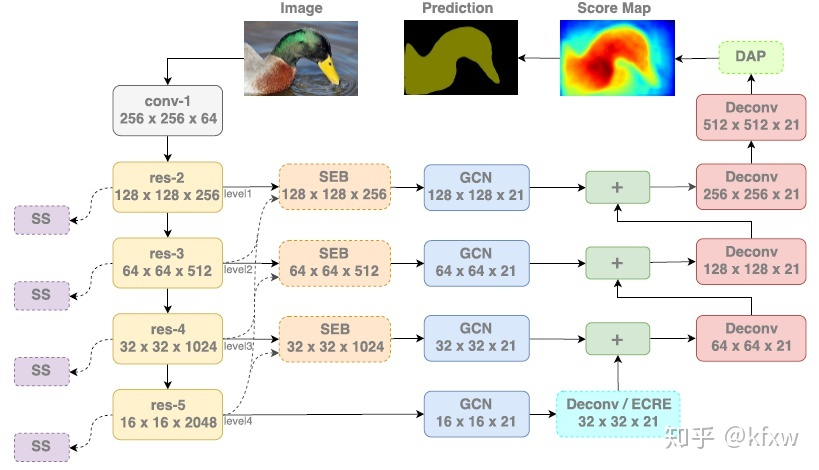
\includegraphics[width=0.95\textwidth]{SemanticSLAM/ExFusion0.jpg}
\caption{ExFusion的实现框图}
\label{ExFusion0}
\end{figure}

其中,SS, SEB, ECRE, DAP是文章作者提出的算法。

\subsubsection{在底层中加入更多的语义信息}
具体是三个方面的改进:
\begin{itemize}
\item Layer Rearrengement

 ResNeXt网络结构中,各级的网络包含的残差单元个数为{3,4,23,3}。为了提高底层特征的语义性,一个想法便是让低层的两级网络拥有的层数更多。因此作者将残差单元个数重排为{8,8,9,8},并重新在ImageNet上预训练模型。重排后网络的分类性能没有明显变化,但是分割模型可以提高约0.8个点(mean intersection over union)的性能。

\item Semantic Supervision(SS)

深度语义监督其实在其他的一些工作里(如GoogLeNet,边缘检测的HED等等)已经使用到了。这里的使用方法基本上没有太大变化,能够带来大约1个点的提升。

\item Semantic Embedding branch(SEB)

\begin{figure}[!hbtp]
\centering
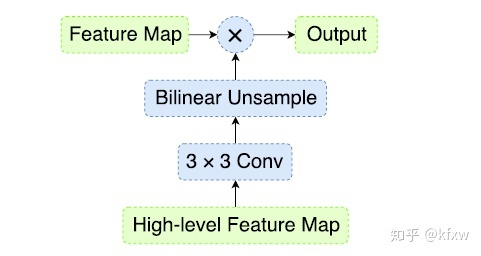
\includegraphics[width=0.65\textwidth]{SemanticSLAM/ExFusion1.jpg}
\caption{语义嵌入分支的结构图}
\label{ExFusion1}
\end{figure}

 其做法是将高层特征上采样后,与低层特征逐像素相乘,用在GCN之前。该部分能带来大约0.7个点的提升。

\end{itemize}

\subsubsection{在高层中加入更多的空间信息}

用两种方法来把更多的空间信息融入到高层特征中:
\begin{itemize}
\item 通道分辨率嵌入(Explicit Channel resolution embedding, ECRE)

其思路是在上采样支路中使用[2,3,4]工作中都使用到的子像素上采样模块(sub-pixel upsample)。作者的出发点并不是前人工作中强调的如速度快、消除反卷积的棋盘效应等等,而是通过这个结构能够让和空间信息相关的监督信息回传到各个通道中,从而让不同通道包含不同空间信息。该模块和原有的反卷积一起使用才能显示出更好的性能。同单独使用反卷积相比,性能可以提高约0.6个点。

\item 稠密邻域预测(Densely adjacent prediction, DAP)

DAP模块只使用在输出预测结果的时候。其想法也是通过扩展通道数来增加空间信息。举一个例子来描述其功能,假设DAP的作用区域为3x3,输出结果的通道数为21,则扩展后的输出通道数为21x3x3。每3x3个通道融合成一个通道。如在最终结果中,第5通道(共21通道)的(12,13)坐标上的像素,是通过DAP之前的第5+0通道(11,12)、5+1通道的(11,13)、5+2通道的(11,14)、5+3通道的(12,12)、5+4通道的(12,13)、5+5通道的(12,14)…平均得到的。DAP能带来约0.6个点的提升。

\end{itemize}

\section{Multi-View Deep Learning for Consistent Semantic Mapping with RGB-D Cameras}

{\color{red} 时间:2018.05.24}







